\documentclass[]{article}
\usepackage{rotating}
\usepackage{booktabs}
\usepackage{lscape} 
\usepackage{graphicx}

\setlength{\pdfpagewidth}{8.5in} \setlength{\pdfpageheight}{11in}

\begin{document}
***back to being too big
%\begin{landscape}
%    \begin{center}
        \scalebox{1}{\begin{table}

\caption{Summary Statistics for Proposed Controls}
\centering
\begin{tabular}[t]{rrrrrrrrrrr}
\toprule
\multicolumn{1}{c}{ } & \multicolumn{2}{c}{Fraction Female} & \multicolumn{2}{c}{Mean Age} & \multicolumn{2}{c}{Fraction At Least 4 Years College} & \multicolumn{2}{c}{Fraction White} & \multicolumn{2}{c}{Mean Income} \\
\cmidrule(l{3pt}r{3pt}){2-3} \cmidrule(l{3pt}r{3pt}){4-5} \cmidrule(l{3pt}r{3pt}){6-7} \cmidrule(l{3pt}r{3pt}){8-9} \cmidrule(l{3pt}r{3pt}){10-11}
Year & Same-Sex & Opposite-Sex & Same-Sex & Opposite-Sex & Same-Sex & Opposite-Sex & Same-Sex & Opposite-Sex & Same-Sex & Opposite-Sex\\
\midrule
2011 & 0.496 & 0.500 & 49.422 & 46.054 & 0.315 & 0.412 & 0.813 & 0.798 & 42767.20 & 47310.34\\
2012 & 0.496 & 0.501 & 49.635 & 46.146 & 0.323 & 0.421 & 0.811 & 0.811 & 44091.95 & 49406.49\\
2013 & 0.495 & 0.499 & 49.809 & 46.975 & 0.327 & 0.413 & 0.807 & 0.804 & 45632.95 & 50450.91\\
2014 & 0.496 & 0.502 & 50.005 & 46.886 & 0.334 & 0.415 & 0.804 & 0.792 & 46754.82 & 52758.57\\
2015 & 0.496 & 0.507 & 50.178 & 46.789 & 0.341 & 0.425 & 0.801 & 0.796 & 48733.81 & 53395.28\\
\addlinespace
2016 & 0.497 & 0.491 & 50.410 & 46.799 & 0.349 & 0.435 & 0.797 & 0.780 & 50181.30 & 55306.73\\
2017 & 0.497 & 0.507 & 50.565 & 46.609 & 0.358 & 0.433 & 0.794 & 0.779 & 51792.06 & 56273.47\\
2018 & 0.497 & 0.499 & 50.689 & 46.305 & 0.363 & 0.440 & 0.791 & 0.771 & 53819.73 & 57059.85\\
2019 & 0.498 & 0.509 & 50.894 & 44.921 & 0.370 & 0.447 & 0.789 & 0.764 & 56634.86 & 58998.77\\
\bottomrule
\end{tabular}
\end{table}
}
%    \end{center}
%\end{landscape}
pretty darn good
WATCH TABLES HAVE BACKWARDS OUTPUT BE CAREFUL
\clearpage

\begin{table}[htbp]

\caption{Summary Statistics for Overall Population}
\label{tab:overall_table}
\centering
\begin{tabular}[t]{rrrr}
\toprule
\multicolumn{2}{c}{ } & \multicolumn{2}{c}{\% in \textit{Obergefell}-legalized States} \\
\cmidrule(l{3pt}r{3pt}){3-4}
Year & \% Same-Sex & Same-Sex & Different-Sex\\
\midrule
2011 & 1 & 90 & 86\\
2012 & 1 & 85 & 80\\
2013 & 1 & 67 & 57\\
2014 & 1 & 37 & 31\\
2015 & 1 & 37 & 32\\
\addlinespace
2016 & 2 & 37 & 32\\
2017 & 2 & 37 & 33\\
2018 & 2 & 37 & 33\\
2019 & 2 & 37 & 34\\
\bottomrule
\end{tabular}
\end{table}

pretty darn good

\clearpage

\begin{landscape}
\begin{center}
\begin{table}

\caption{Individuals by Location}
\centering
\begin{tabular}[t]{rrrrrrrrrrr}
\toprule
\multicolumn{1}{c}{ } & \multicolumn{2}{c}{In Locally Legalized} & \multicolumn{2}{c}{Migrants in Locally Legalized} & \multicolumn{1}{c}{ } & \multicolumn{2}{c}{In from Locally Legalized} & \multicolumn{2}{c}{Migrants from Locally Legalized} & \multicolumn{1}{c}{ } \\
\cmidrule(l{3pt}r{3pt}){2-3} \cmidrule(l{3pt}r{3pt}){4-5} \cmidrule(l{3pt}r{3pt}){7-8} \cmidrule(l{3pt}r{3pt}){9-10}
Year & Same-Sex & Opposite-Sex & Same-Sex & Opposite-Sex & Difference & Same-Sex & Opposite-Sex & Same-Sex & Opposite-Sex & Difference\\
\midrule
2011 & 0.151 & 0.111 & 0.144 & 0.084 & 0.060 & 0.151 & 0.111 & 0.089 & 0.146 & 0.057\\
2012 & 0.223 & 0.184 & 0.192 & 0.157 & 0.035 & 0.223 & 0.185 & 0.163 & 0.193 & 0.029\\
2013 & 0.468 & 0.404 & 0.434 & 0.372 & 0.061 & 0.470 & 0.406 & 0.384 & 0.445 & 0.060\\
2014 & 0.712 & 0.672 & 0.679 & 0.655 & 0.024 & 0.712 & 0.673 & 0.664 & 0.683 & 0.019\\
2015 & 0.706 & 0.670 & 0.676 & 0.650 & 0.026 & 0.705 & 0.671 & 0.660 & 0.669 & 0.010\\
\addlinespace
2016 & 0.703 & 0.670 & 0.673 & 0.653 & 0.019 & 0.703 & 0.671 & 0.663 & 0.672 & 0.010\\
2017 & 0.700 & 0.670 & 0.667 & 0.650 & 0.017 & 0.701 & 0.671 & 0.658 & 0.676 & 0.018\\
2018 & 0.698 & 0.670 & 0.667 & 0.653 & 0.014 & 0.700 & 0.671 & 0.664 & 0.678 & 0.014\\
2019 & 0.684 & 0.668 & 0.641 & 0.650 & -0.010 & 0.684 & 0.669 & 0.660 & 0.641 & -0.019\\
\bottomrule
\end{tabular}
\end{table}

\end{center}
\end{landscape}
some size issues but could be worse

\clearpage

\begin{landscape}
\begin{center}
\begin{table}

\caption{Migration Trends Data}
\centering
\begin{tabular}[t]{rrrrrrrrrrrrr}
\toprule
\multicolumn{1}{c}{ } & \multicolumn{6}{c}{Fraction Moving To} & \multicolumn{6}{c}{Fraction Moving From} \\
\cmidrule(l{3pt}r{3pt}){2-7} \cmidrule(l{3pt}r{3pt}){8-13}
\multicolumn{1}{c}{ } & \multicolumn{2}{c}{Same-Sex} & \multicolumn{1}{c}{ } & \multicolumn{2}{c}{Opposite-Sex} & \multicolumn{1}{c}{ } & \multicolumn{2}{c}{Same-Sex} & \multicolumn{1}{c}{ } & \multicolumn{2}{c}{Opposite-Sex} & \multicolumn{1}{c}{ } \\
\cmidrule(l{3pt}r{3pt}){2-3} \cmidrule(l{3pt}r{3pt}){5-6} \cmidrule(l{3pt}r{3pt}){8-9} \cmidrule(l{3pt}r{3pt}){11-12}
Year & Locally Legalized & Federally Legalized & Difference & Locally Legalized & Federally Legalized & Difference & Locally Legalized & Federally Legalized & Difference & Locally Legalized & Federally Legalized & Difference\\
\midrule
2011 & 0.156 & 0.163 & -0.007 & 0.078 & 0.105 & -0.027 & 0.157 & 0.163 & -0.006 & 0.081 & 0.104 & -0.023\\
2012 & 0.146 & 0.170 & -0.025 & 0.087 & 0.106 & -0.020 & 0.138 & 0.172 & -0.034 & 0.090 & 0.106 & -0.016\\
2013 & 0.164 & 0.177 & -0.014 & 0.099 & 0.111 & -0.012 & 0.167 & 0.175 & -0.008 & 0.102 & 0.109 & -0.008\\
2014 & 0.160 & 0.177 & -0.017 & 0.105 & 0.113 & -0.008 & 0.158 & 0.182 & -0.025 & 0.106 & 0.111 & -0.005\\
2015 & 0.165 & 0.184 & -0.019 & 0.105 & 0.113 & -0.008 & 0.161 & 0.191 & -0.030 & 0.106 & 0.111 & -0.004\\
\addlinespace
2016 & 0.170 & 0.186 & -0.016 & 0.105 & 0.111 & -0.006 & 0.170 & 0.186 & -0.016 & 0.107 & 0.109 & -0.003\\
2017 & 0.158 & 0.183 & -0.025 & 0.104 & 0.112 & -0.007 & 0.159 & 0.180 & -0.020 & 0.106 & 0.110 & -0.004\\
2018 & 0.174 & 0.195 & -0.021 & 0.104 & 0.109 & -0.005 & 0.177 & 0.189 & -0.012 & 0.105 & 0.107 & -0.001\\
2019 & 0.169 & 0.209 & -0.039 & 0.102 & 0.107 & -0.005 & 0.169 & 0.209 & -0.041 & 0.103 & 0.105 & -0.002\\
\bottomrule
\end{tabular}
\end{table}

\end{center}
\end{landscape}
PERFECT

\clearpage

\begin{figure}
    \centering
    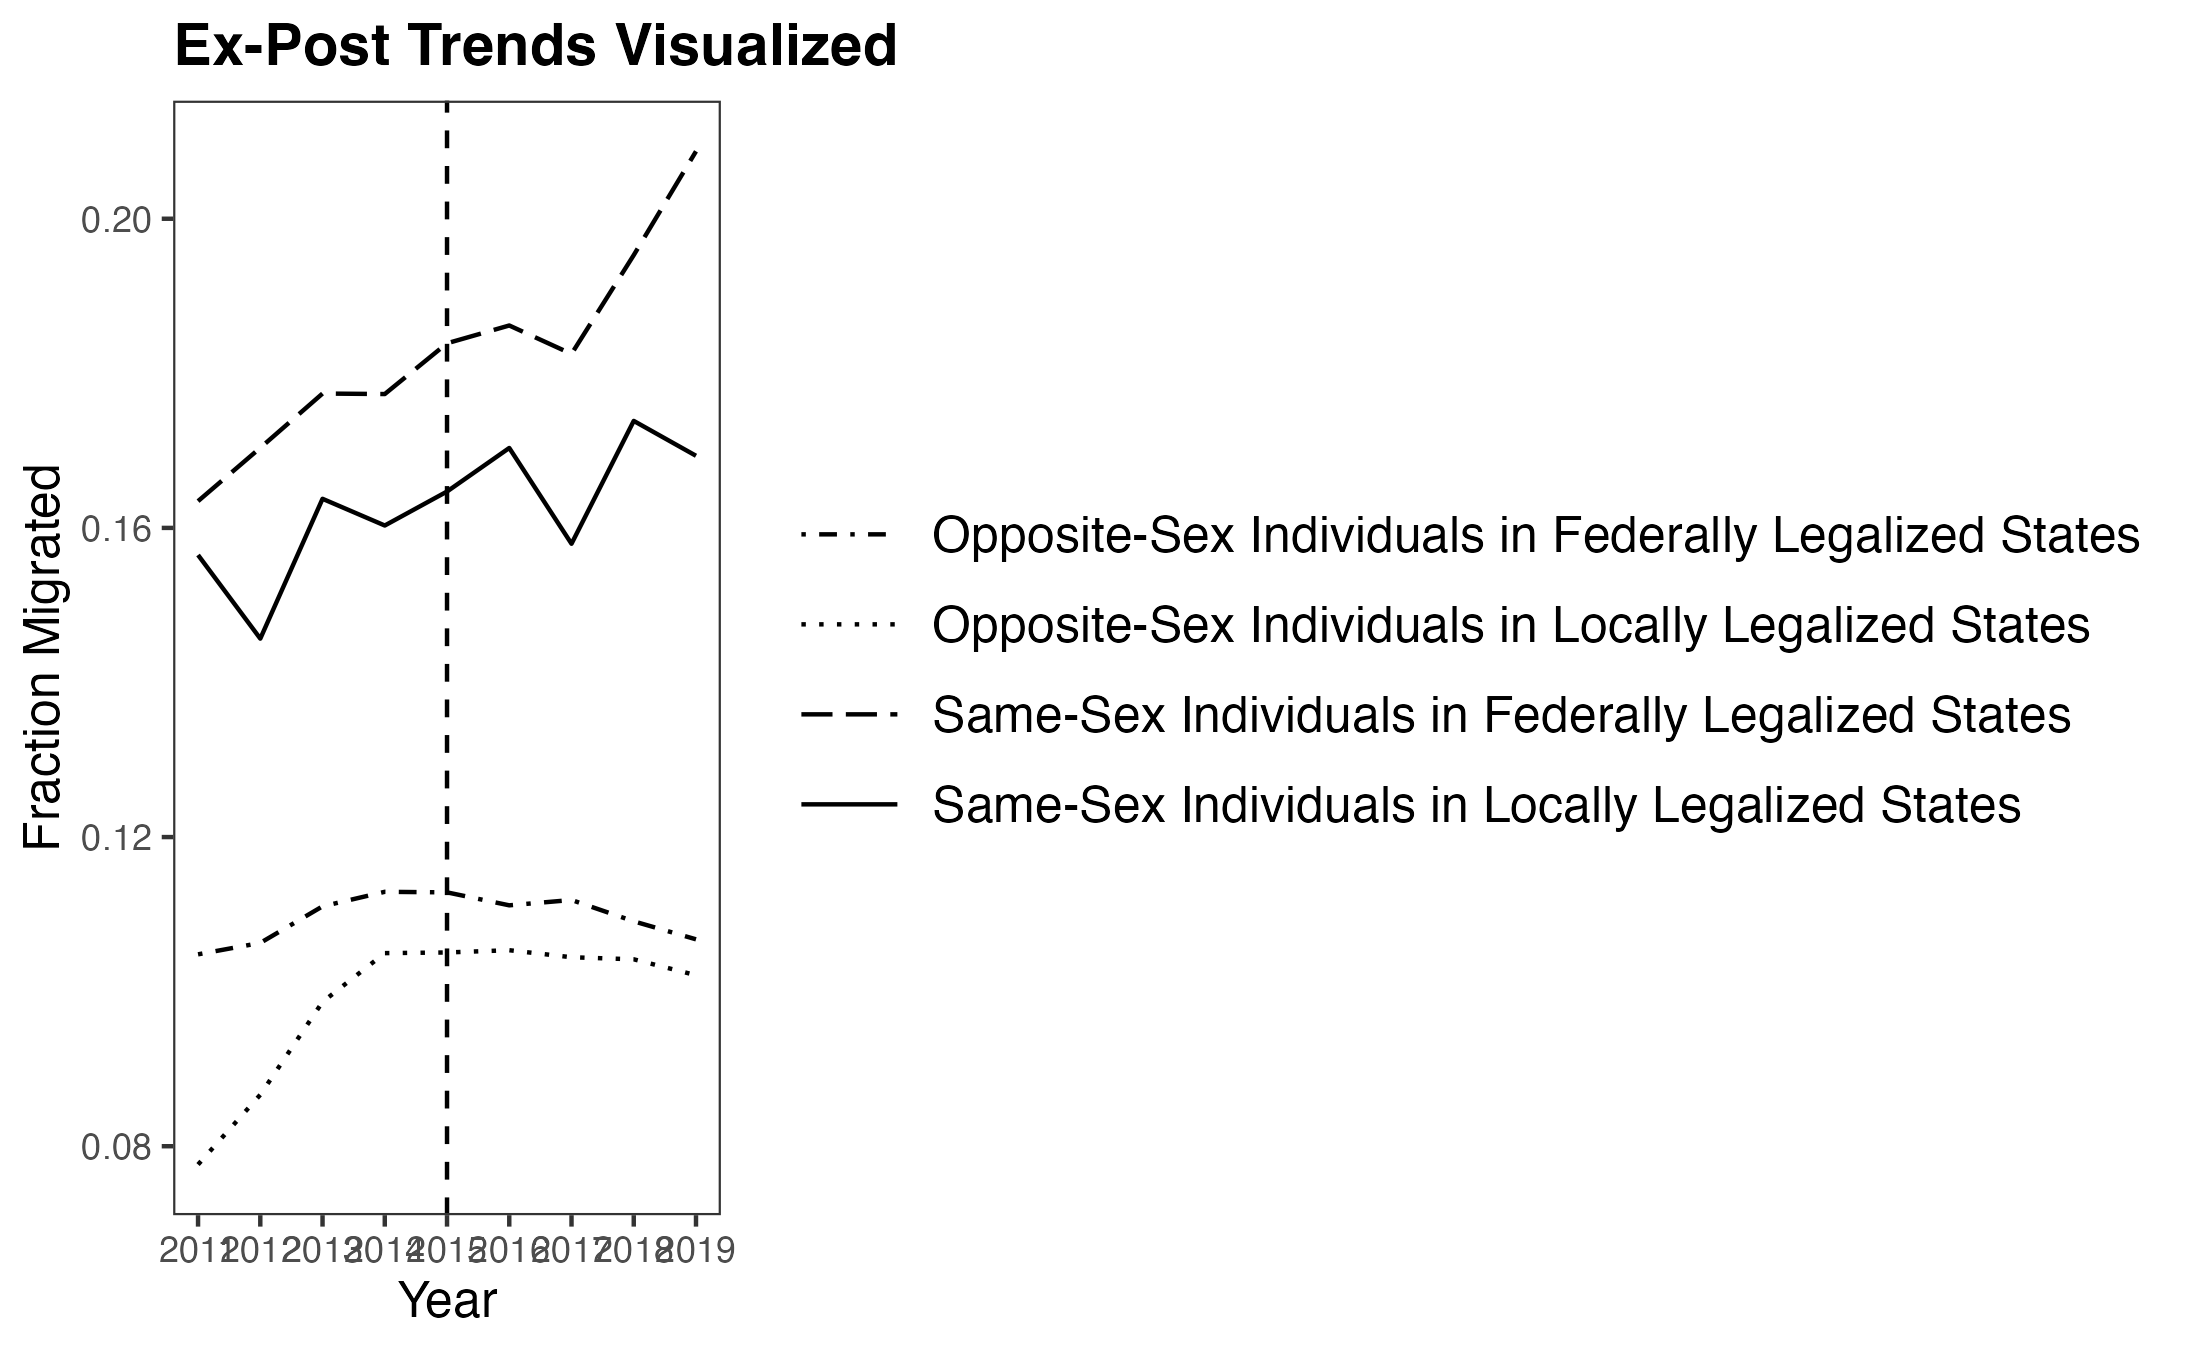
\includegraphics[width=1\linewidth]{outputs/summary_stats/post_trends.png}
    \caption{Enter Caption}
    \label{fig:enter-label}
\end{figure}

\begin{figure}
    \centering
    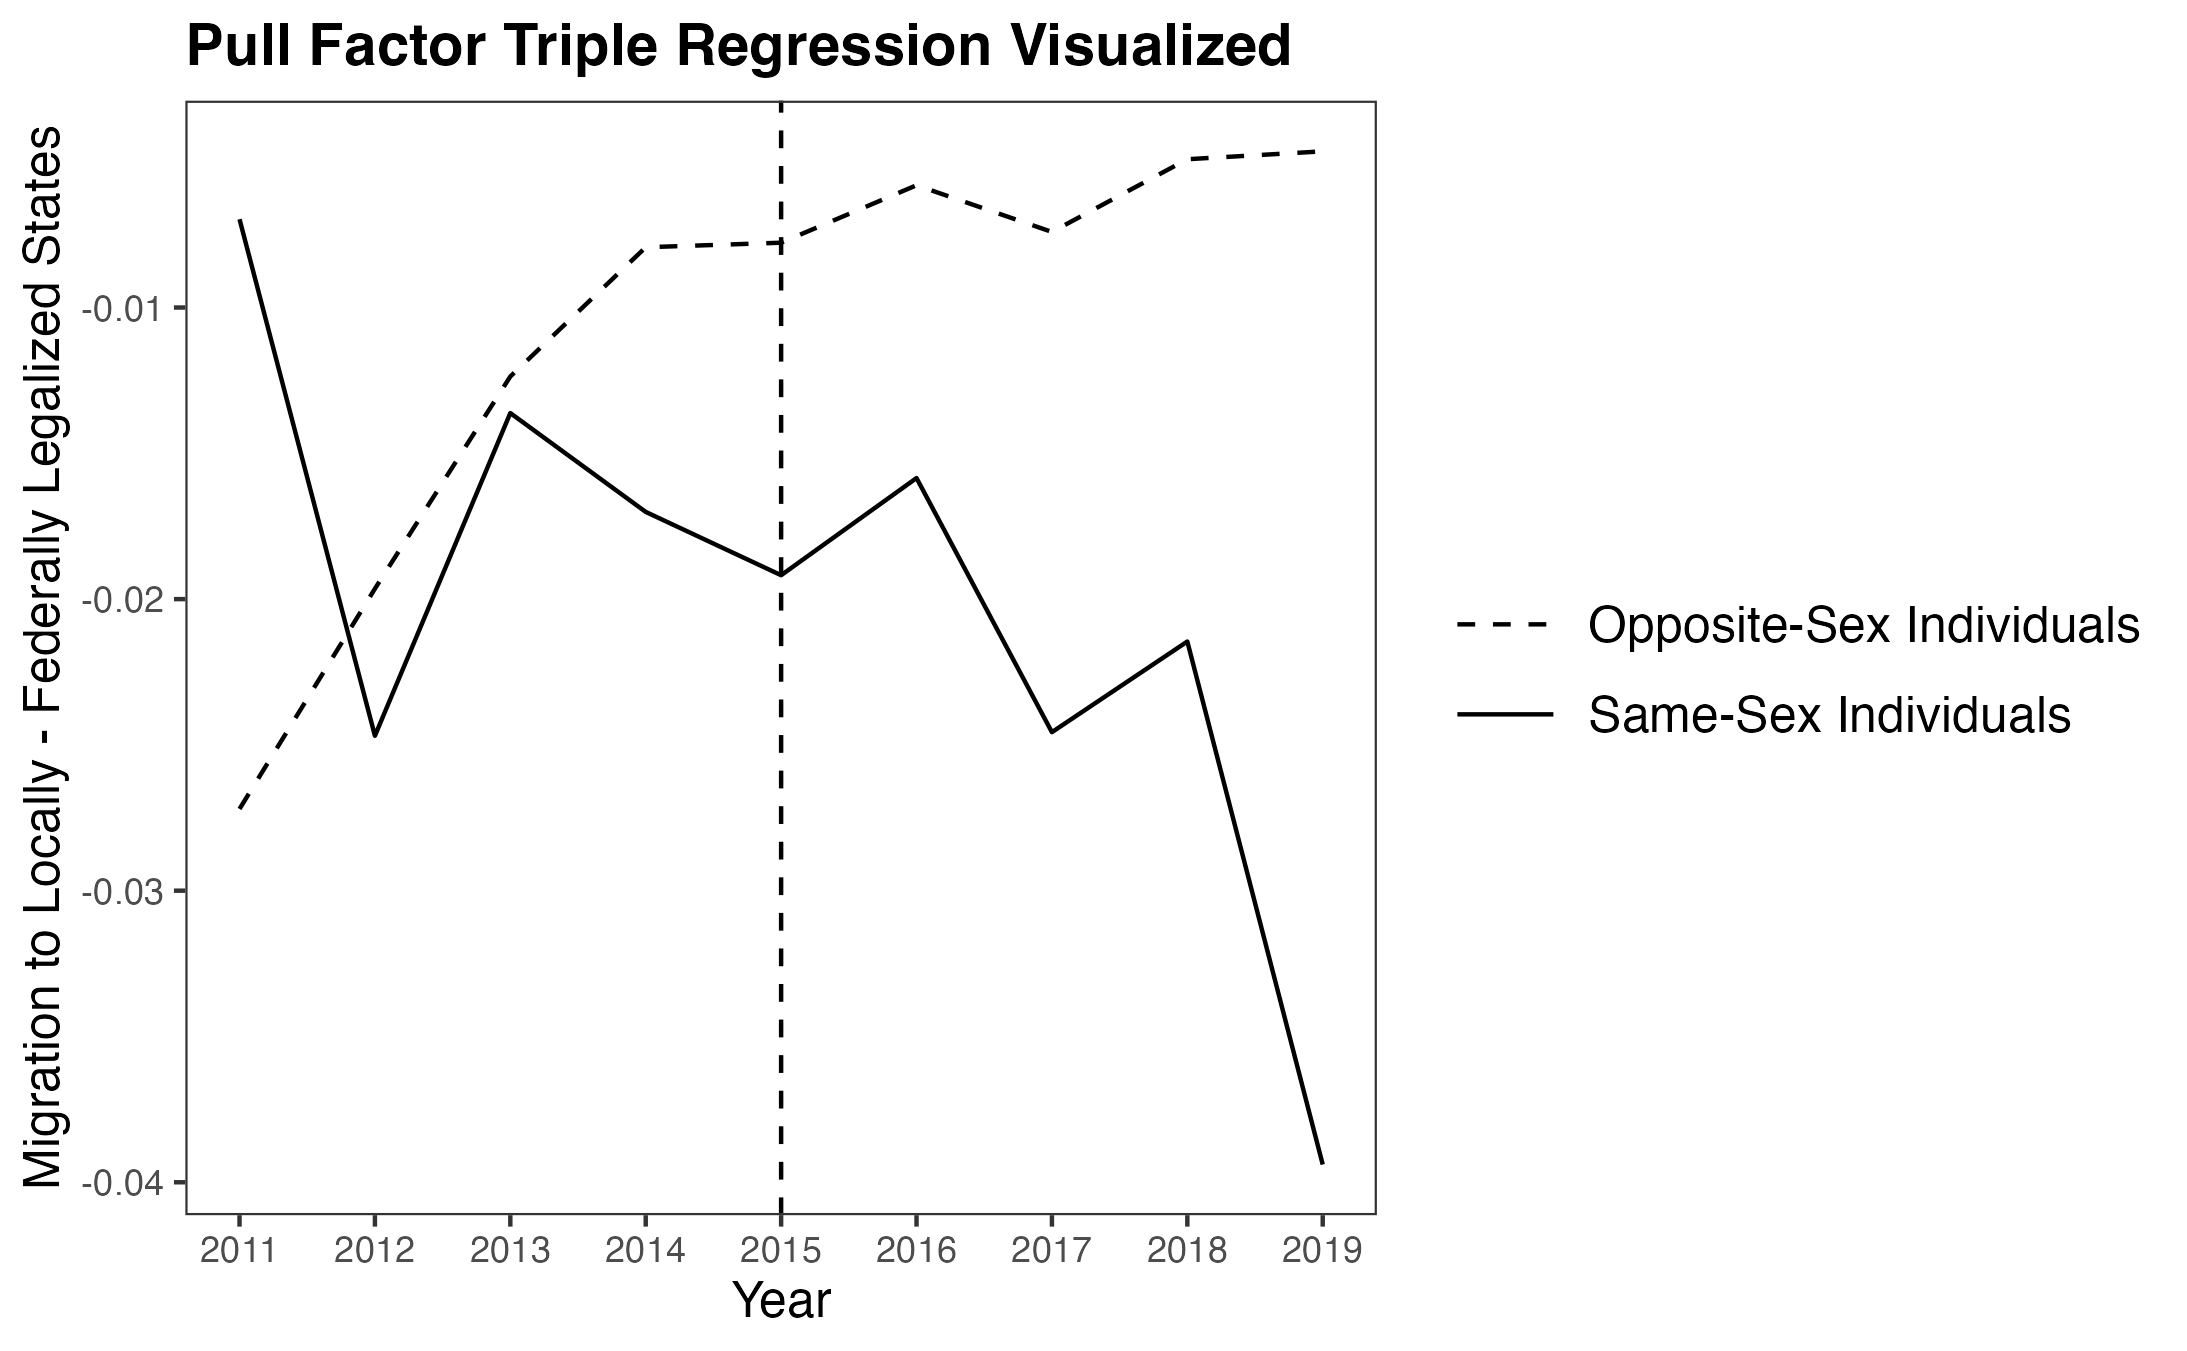
\includegraphics[width=1\linewidth]{outputs/summary_stats/post_diffs.png}
    \caption{Enter Caption}
    \label{fig:enter-label}
\end{figure}

\begin{figure}
    \centering
    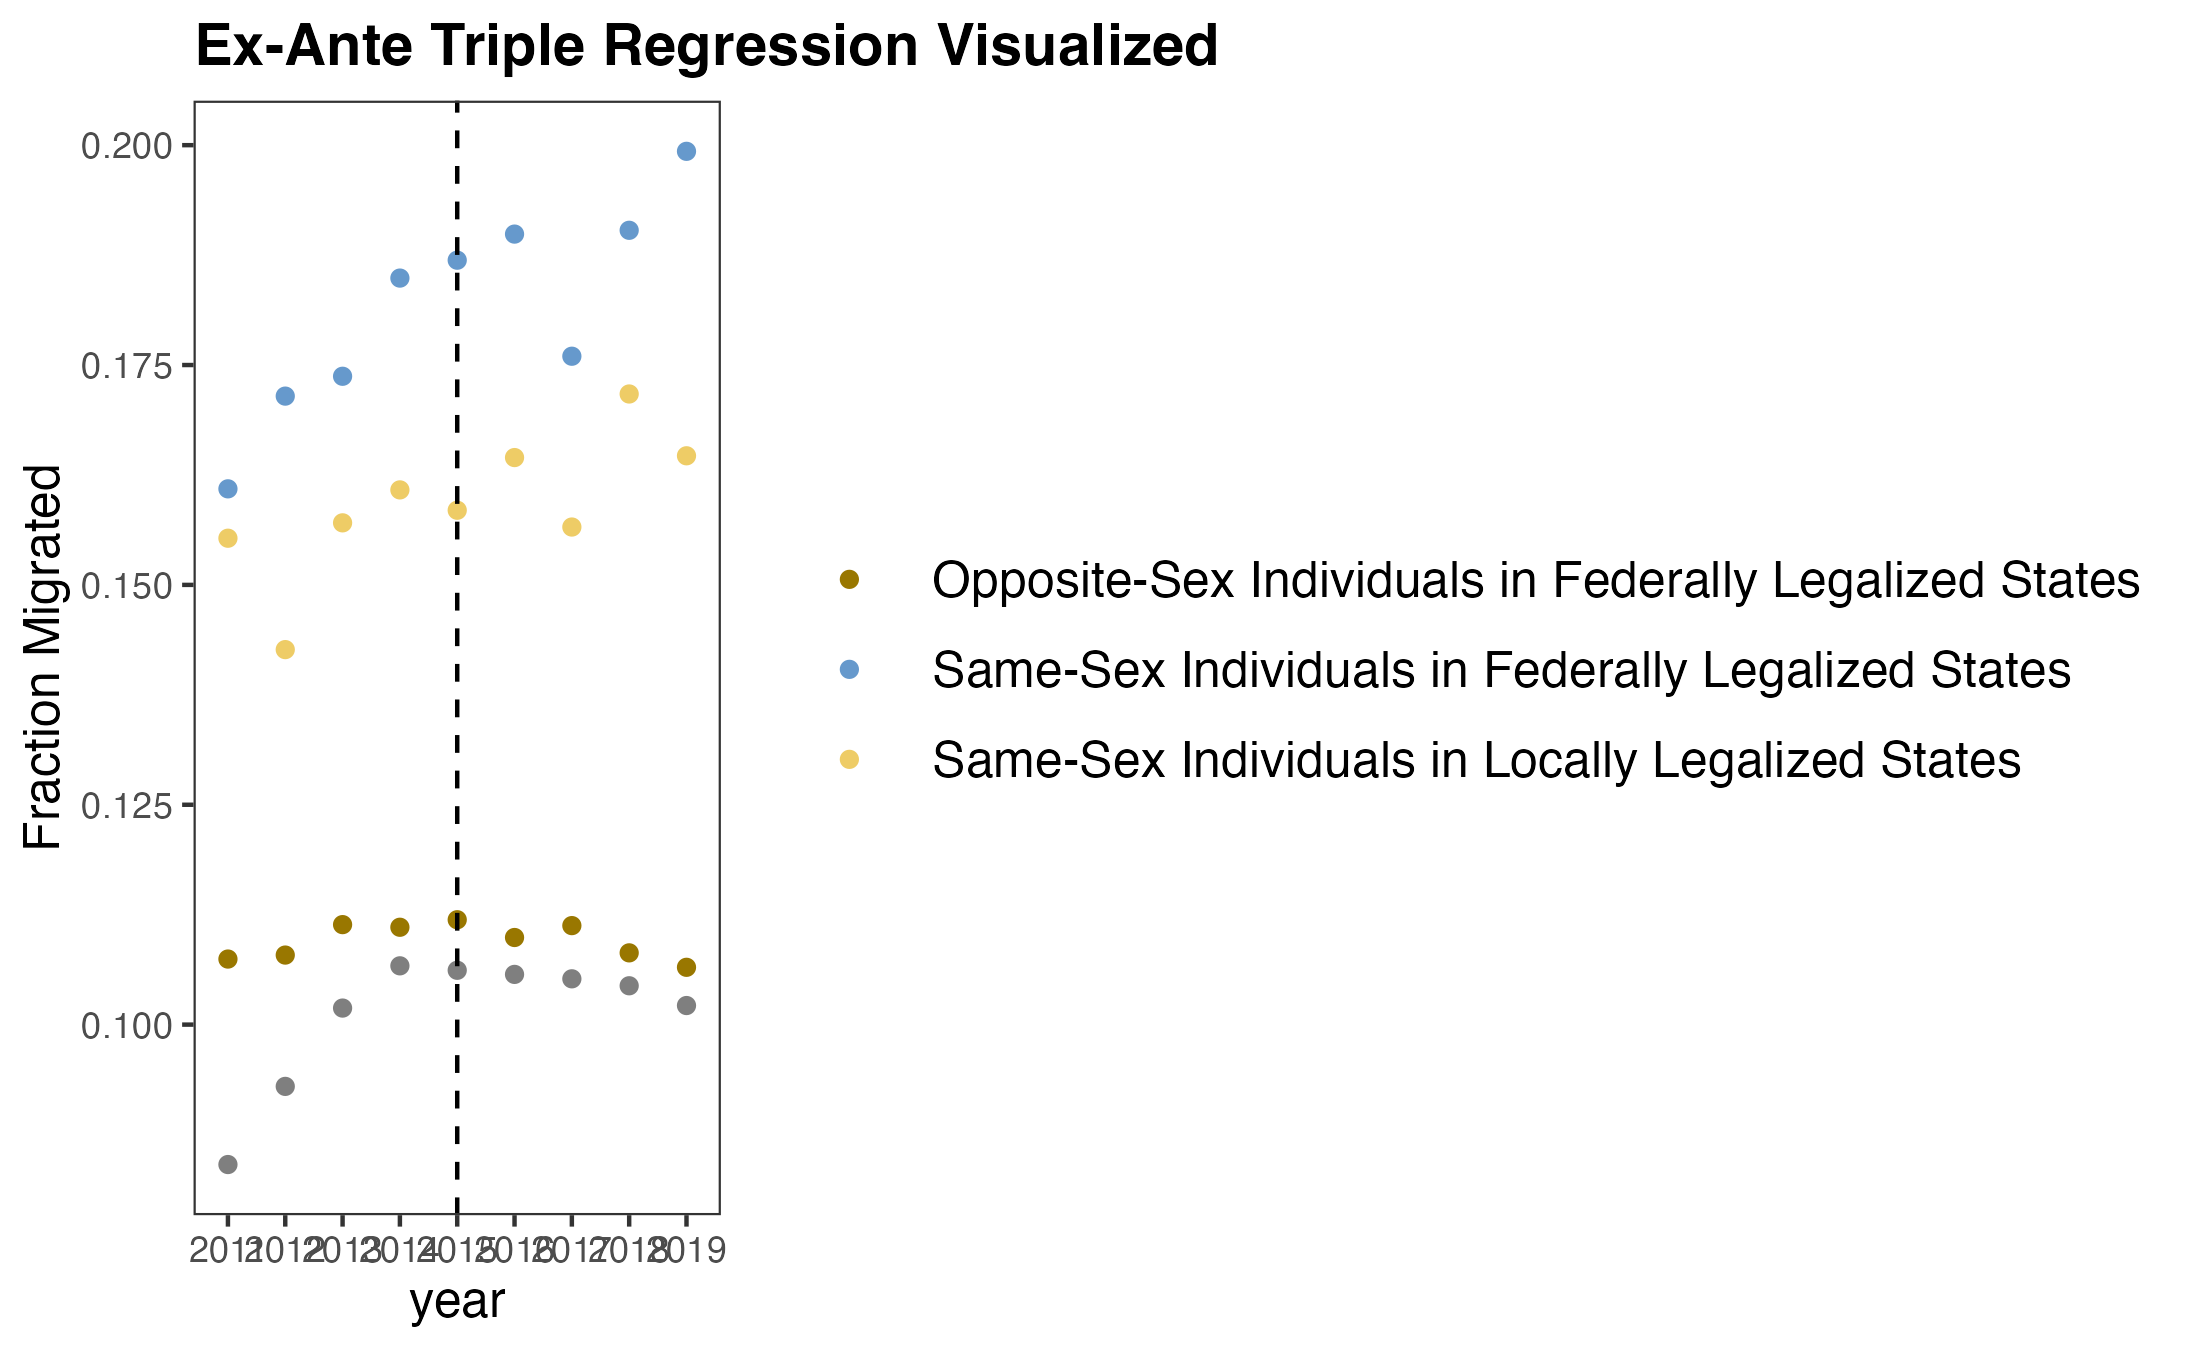
\includegraphics[width=1\linewidth]{outputs/summary_stats/ante_trends.png}
    \caption{Enter Caption}
    \label{fig:enter-label}
\end{figure}

\begin{figure}
    \centering
    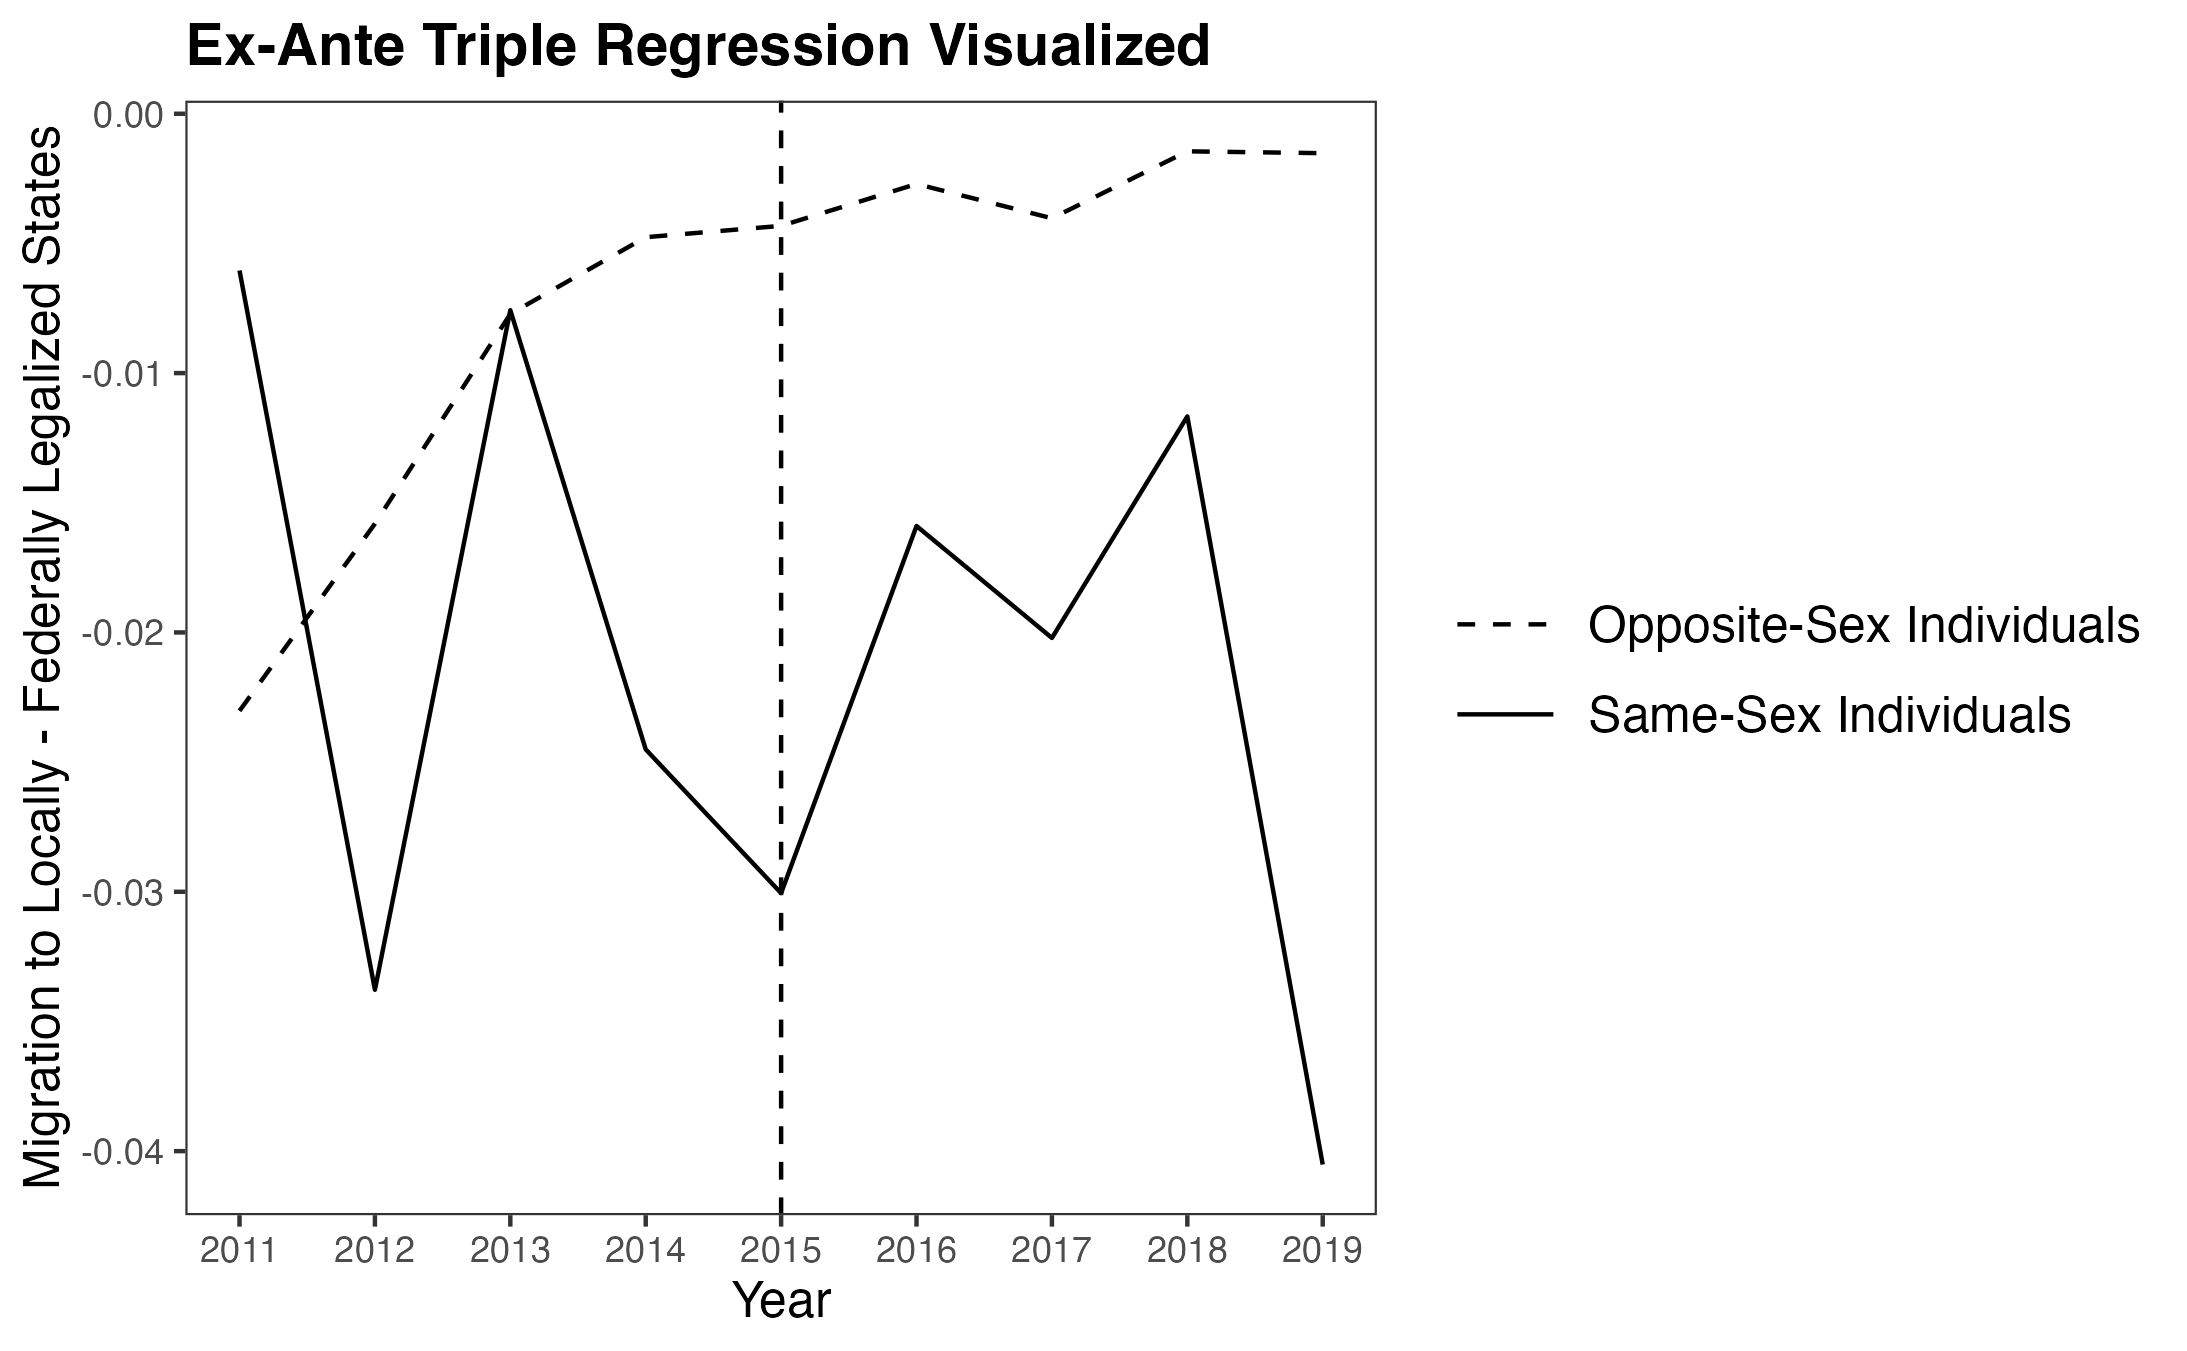
\includegraphics[width=1\linewidth]{outputs/summary_stats/ante_diffs.png}
    \caption{Enter Caption}
    \label{fig:enter-label}
\end{figure}
Ok some squashing, formatting consistency issues but can work with


\clearpage

\begin{tabular}{lccc}
\multicolumn{4}{c}{Ex-Post Model} \\ \hline
 & (1) & (2) & (3) \\
VARIABLES & migrant & migrant & migrant \\ \hline
 &  &  &  \\
1.in\_samesex\#1.expost\_old\_legal\#1.post\_2015 & -0.015* & -0.013* & 0.013 \\
 & (0.007) & (0.006) & (0.033) \\
Constant & 0.106*** & 0.394*** & 3.356*** \\
 & (0.001) & (0.008) & (0.080) \\
 &  &  &  \\
Observations & 956,236,912 & 956,236,912 & 956,236,912 \\
 R-squared & 0.004 & 0.070 & 0.921 \\ \hline
\multicolumn{4}{c}{ Robust standard errors in parentheses} \\
\multicolumn{4}{c}{ *** p$<$0.01, ** p$<$0.05, * p$<$0.1} \\
\multicolumn{4}{c}{ Model 1 includes interaction terms and fixed effects only.} \\
\multicolumn{4}{c}{ )} \\
\multicolumn{4}{c}{ )} \\
\multicolumn{4}{c}{ )} \\
\multicolumn{4}{c}{ )} \\
\end{tabular}


temporary place for description of models:
Model 1 includes interaction terms and fixed effects only. Model 2 includes interaction terms, fixed effects, and controls for sex, race, education, age and income. Model 3 includes interaction terms, fixed effects, and controls for sex, race, education, age, income, and birthstate. Models 1 and 2 use a weighted sample. Model 3 uses a weighted and collapsed sample.

\clearpage

\begin{tabular}{lccc}
\multicolumn{4}{c}{Ex-Ante Model} \\ \hline
 & (1) & (2) & (3) \\
VARIABLES & migrant & migrant & migrant \\ \hline
 &  &  &  \\
1.in\_samesex\#1.exante\_old\_legal\#1.post\_2015 & -0.016 & -0.014 & 0.014 \\
 & (0.009) & (0.008) & (0.030) \\
Constant & 0.106*** & 0.394*** & 3.757*** \\
 & (0.001) & (0.007) & (0.123) \\
 &  &  &  \\
Observations & 956,236,912 & 956,236,912 & 956,236,912 \\
 R-squared & 0.003 & 0.069 & 0.912 \\ \hline
\multicolumn{4}{c}{ Robust standard errors in parentheses} \\
\multicolumn{4}{c}{ *** p$<$0.01, ** p$<$0.05, * p$<$0.1} \\
\multicolumn{4}{c}{p{\textwidth}}{ Model 1 includes interaction terms and fixed effects only. \newline
Model 2 includes interaction terms, fixed effects, and controls for sex, race, education, age, and income. \newline
Model 3 includes interaction terms, fixed effects, and controls for sex, race, education, age, income, and birthstate. \newline
Models 1 and 2 use a weighted sample. Model 3 uses a weighted and collapsed sample.} \\
\multicolumn{4}{c}{ )} \\
\multicolumn{4}{c}{ )} \\
\multicolumn{4}{c}{ )} \\
\multicolumn{4}{c}{ )} \\
\end{tabular}

temporary place for description of models:
Model 1 includes interaction terms and fixed effects only. Model 2 includes interaction terms, fixed effects, and controls for sex, race, education, age and income. Model 3 includes interaction terms, fixed effects, and controls for sex, race, education, age, income, and birthstate. Models 1 and 2 use a weighted sample. Model 3 uses a weighted and collapsed sample.
\clearpage
\hspace{-4cm}
\begin{tabular}{lcccc}
\multicolumn{5}{c}{Ex-Post Model} \\ \hline
 & (1) & (2) & (3) & (4) \\
VARIABLES & Local To Local & Local To Federal & Federal To Local & Federal To Federal \\ \hline
 &  &  &  &  \\
1.in\_samesex\#1.expost\_old\_legal\#1.post\_2015 & 0.006 & -0.001 & -0.003 & -0.016** \\
 & (0.004) & (0.001) & (0.003) & (0.006) \\
Constant & -0.001 & 0.010*** & -0.001** & 0.099*** \\
 & (0.002) & (0.001) & (0.000) & (0.003) \\
 &  &  &  &  \\
Observations & 956,236,912 & 956,236,912 & 956,236,912 & 956,236,912 \\
 R-squared & 0.054 & 0.009 & 0.004 & 0.057 \\ \hline
\multicolumn{5}{c}{ Robust standard errors in parentheses} \\
\multicolumn{5}{c}{ *** p$<$0.01, ** p$<$0.05, * p$<$0.1} \\
\multicolumn{5}{c}{ Only has state and year fixed effects.} \\
\end{tabular}


\hspace{-4cm}
\begin{tabular}{lcccc}
\multicolumn{5}{c}{Ex-Post Model} \\ \hline
 & (1) & (2) & (3) & (4) \\
VARIABLES & Local To Local & Local To Federal & Federal To Local & Federal To Federal \\ \hline
 &  &  &  &  \\
1.in\_samesex\#1.exante\_old\_legal\#1.post\_2015 & 0.006 & -0.003 & -0.003** & -0.016** \\
 & (0.004) & (0.003) & (0.001) & (0.006) \\
Constant & -0.000 & -0.001* & 0.008*** & 0.100*** \\
 & (0.002) & (0.000) & (0.000) & (0.002) \\
 &  &  &  &  \\
Observations & 956,236,912 & 956,236,912 & 956,236,912 & 956,236,912 \\
 R-squared & 0.053 & 0.005 & 0.006 & 0.057 \\ \hline
\multicolumn{5}{c}{ Robust standard errors in parentheses} \\
\multicolumn{5}{c}{ *** p$<$0.01, ** p$<$0.05, * p$<$0.1} \\
\multicolumn{5}{c}{ Only has state and year fixed effects.} \\
\end{tabular}


\clearpage

\begin{landscape}
\small
\begin{tabular}{lc}
\multicolumn{2}{c}{Ex-Post Model by Sex} \\ \hline
 & (1) \\
VARIABLES & Model 1: Men \\ \hline
 &  \\
1.in\_samesex\#1.expost\_old\_legal\#1.post\_2015 & -0.005*** \\
 & (0.001) \\
Constant & 0.106*** \\
 & (0.001) \\
 &  \\
Observations & 481,915,892 \\
 R-squared & 0.004 \\ \hline
\multicolumn{2}{c}{ Robust standard errors in parentheses} \\
\multicolumn{2}{c}{ *** p$<$0.01, ** p$<$0.05, * p$<$0.1} \\
\multicolumn{2}{c}{ See below.} \\
\end{tabular}

\end{landscape}

\clearpage
\begin{landscape}
\begin{tabular}{lcc}
\multicolumn{3}{c}{Ex-Ante Model} \\ \hline
 & (1) & (2) \\
VARIABLES & Model 1: Male & Model 1: Female \\ \hline
 &  &  \\
ante\_treatment & -0.005 & -0.010 \\
 & (0.010) & (0.013) \\
Constant & 0.185*** & 0.186*** \\
 & (0.000) & (0.000) \\
 &  &  \\
Observations & 481,915,892 & 474,321,020 \\
 R-squared & 0.004 & 0.004 \\ \hline
\multicolumn{3}{c}{ Robust standard errors in parentheses} \\
\multicolumn{3}{c}{ *** p$<$0.01, ** p$<$0.05, * p$<$0.1} \\
\multicolumn{3}{c}{ See below.} \\
\end{tabular}

\end{landscape}
\end{document}




